\chapter{Image Filtering}

\section{Image Types and Discretization}

Definition of continuous grey-scale image: \emph{Mapping f from a rectangular domain $\Omega = (0,w) \times (0,h)$ to a co-domain $\mathbb{R}$, $f : \mathbb{R}^2 \supset \Omega \rightarrow \mathbb{R}$}, $\Omega$ is called image domain/plane and $\mathbb{R}$ specifies grey value.

\textbf{Sampling}

Sampling $\Omega$ gives $(f_{i,j})_{i=1,\dots ,N, j=1, \dots , M}$, $i,j$ being pixel elements. Coarse sampling leads to bad image quality (LS 1.6).

Low sampling rates create \textit{aliasing}, i.e., signals are indistinguishable when sampled. From DSP we know that sampling rate has to be greater than nyquist rate (highest frequency in domain).

\textbf{Quantisation}

Discretization of co-domain, i.e., grey value, for instance $\{0,1,...,255\}$ encoded by a byte. Visualization depicted in LS 1.9.

\textbf{m-Dimensional images}

Domain is now $\mathbb{R}^m$, m=1: Signals, m=2: 2D images, m=3: 3D images.

\textbf{Vector-valued images}

I.e., three channel RGB images (color images), hence co-domain is in $\mathbb{R}^n$. Also sattelite images, having multispectral images with different frequency bands.

\textbf{Matrix-valued images}

Sometime called "tensor". Co-domain: $\mathbb{R}^{n\times n}$, Example: "diffusion tensor MRI", for each voxel in 3D image has a symmetric $3\times 3$ matrix. Example images on LS 1.15.

\textbf{Image sequences}

All of the former examples, can be extended by one dimension so that we have a sequence of mages, i.e., a video.

\textbf{Relevant images}

Focus on 2D scalar or RGB images. Gradient of greyscale images also important (m=2, n=2), Tensors also important.

\textbf{Notations}:

Greyscale: $f = (f_{i,j}), f_{i,j} \in \mathbb{R}$, $i,j$ pixel coordinates.

RGB: $\textbf{f} : \mathbb{Z}^2 \rightarrow \mathbb{R}^3$, bold-faced letter f.

\section{Image noise}

\textbf{Types of noise:}

\begin{itemize}
    \item Additive Noise
    \item Multiplicative Noise
    \item Impulse Noise
    \item Salt and pepper Noise
\end{itemize}

\subsection{Additive Noise}
Most important type. Greyvalues and noise assumed independent, i.e., $$f_{i,j} = g_{i,j}+n_{i,j}$$, $g$ original values, $n$ noise values. Noise may have different distributions.

\textbf{Uniform distribution:} Often not realistic, easy simulation. Constant density function within interval $[a,b]$: $p(x) = b-a, x \in [a,b]$. Can appear due to quantisation when discretizing an image.

Example: \begin{verbatim}
g = ones ( [512 ,512] )*128;
	a = -64; b = 64;
	n = a + ( b-a) * rand ( size ( image ) ) ;
	f = g + n ;
	figure ,
	subplot (1 ,2 ,1)
	imshow( f / 255.0) ,
	subplot (1 ,2 ,2)
	imhist ( uint 8 ( f ) )
\end{verbatim}

\textbf{Gaussian distribution:} Most important noise model. Good approx. in many applications. Density function: $$p(x) = \dfrac{1}{\sqrt{2\pi \sigma^2}} e^{-\dfrac{(x - \mu)^2}{2\sigma^2}}$$. In the end it looks like the "Bell curve". $\mu - 2\sigma$ to $\mu + 2\sigma$ includes 95.5\% of the values (significance interval).

\subsection{Multiplicative Noise}

Signal-dependent unlike add. noise. Often proportional to grey value: $$f_{i,j} = g _{i,j} + n_{i,j}g_{i,j} = (1+n_{i,j}) g_{i,j}$$ and can of course follow different distributions.

Prevalent in Radar, Ultrasound, Tomographic images. Example of gaussian mult. noise is on LS 1.31.

\subsection{Impulse Noise}

Only effects some pixels, can appear due to defects in camera for instance. \textbf{Unipolar impulse noise} degrations only have one grey value, \textbf{Bipolar noise} deg. have two. \textbf{Bipolar noise} with highest and lowest grey values is called \textbf{Salt and Pepper Noise}! (Example on LS 1.33).

\section{Correlation and Convolution}

How to get rid of noise? Given camera and still scene, take mult. images and calculate average. What if you only have one image?

\textbf{Idea:} Modify pixel according to neighborhood of the pixel. Simple solution: use average of neighbors for pixel, also called moving average.

Kernel for moving average: $\dfrac{[1_1, \dots, 1_N]}{N}$ (in 1D, i.e., signals).

Moving average in 2D: Place "box" over a pixel with dim. $n\times m$, then you have $n\cdot m$ values for average computation (Example on LS 1.40).

\subsection{Correlation}
Generalization of the previous approach: weighted combination of pixels in small neighborhoods. Formally: $$g_{i,j} = \sum\limits_{k,l \in \mathbb{Z}} f_{i+k,j+l} h_{k,l} = f \otimes h$$, entries of kernel are called \textbf{filter coefficients}, $\otimes$ being the correlation operator.

\textbf{Smoothing with a box}: Leads to "line-like" artifacts, no smooth border.

\textbf{Boundary conditions:} Dark borders are the result of not having special boundary conditions, since pixels are just used with 0 value without boundary conditions.

\begin{description}
    \item[zero] Standard zero-padding, dark borders
    \item[wrap] "Repeat" the whole image at the borders
    \item[clamp] Only repeat the border-pixels
    \item[mirror] "Mirror" the image at the borders
\end{description}

\subsection{Gaussian filter}

Goal: nearest neighbor pixels have more influence. Calculate Kernel weights according to gaussian distribution. In 2D the formular is $$h(u,v) = \dfrac{1}{\sqrt{2\pi \sigma^2}} e^{-\dfrac{u^2 - v^2}{2\sigma^2}}$$. As a result, values close to the center of the box are higher than outside.

Gives better results and no artifacts. $\sigma$ and the size of the kernel, determine how strongly the image is "smoothed". Bigger $\sigma$, smoother image. Examples are on LS 1.47 to 1.50.

\subsection{Convolution}

Impulse response of correlation shows, that filter is flipped, there is no left-side "identity element" and that it is not commutative. Better: \textbf{Convolution}.

It is equivalent to flipping the filter left-right, to-bottom. Notation: $g = f * h$ and the formular is $$g_{i,j} = \sum\limits_{k,l \in \mathbb{Z}} f_{i-k,j-l} h_{k,l}$$ and the impulse response $\delta * h = h$, which is also called \textit{impulse response function}. Symmetric filters in both dimensions have same results for corr. and conv.

\textbf{Properties}
\begin{itemize}
    \item Commutative
    \item Associative
    \item Identity element
    \item Linear (constant factor scaling and additive)
    \item Shift-invariant
\end{itemize}

\subsection{Sharpening}
When subtracting a blurred image from the original, we get some kind of edge highlight. Adding it back, sharpens the picture (LS 1.56).

\textbf{Sharpening noise is bad}: Noise is high frequency, and adding back high frequency amplifies noise.

\section{Non-Linear Filters and Denoising}

Example on LS 1.65 shows that denoising gaussian noise with gaussian filter can have subjectively bad result. How to measure "how good" it is? Two measures:

\textbf{Mean Square Error} $$MSE(f,g) = \frac{1}{N} \sum\limits_{n=1}^N (f_n - g_n)^2$$
\textbf{Peak signal-to-noise ratio (PSNR)} $$PSNR(f,g) = 10 \log_{10} \left(\dfrac{V^2}{MSE(f,g)}\right)$$

Trying different parameters, the one with the highest PSNR will have the best result. The result is still bad with edges, gaussian filter may not be too good for denoising gaussian noise.

\subsection{Bilateral Filter}  

\textbf{Idea:} To preserve edges, average over pixels nearby with similar color. Two weights: \textbf{distance} and \textbf{intensity}. Visually:

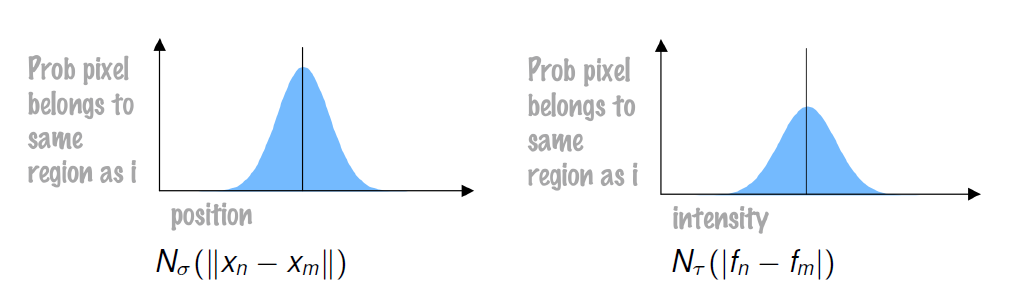
\includegraphics[width=\textwidth]{images/chap1/bilateral}, $x_n,x_m$ being pixel positions and $f_n, f_m$ pixel intensities, $\sigma, \tau$ the standard deviation for the two gaussian dists. $N_\sigma, N_\tau$. The filter in $n$-th pixel is defined as: $$g(n) = \dfrac{1}{K_n} \sum\limits_{m=1}^N f_m N_\sigma(||x_n - x_m||) N_\tau (|f_n -f_m|)$$ with $$K_n = \sum\limits_{m=1}^N N_\sigma(||x_n - x_m||) N_\tau (|f_n -f_m|)$$.

Sum is defined over all pixels, usually only small window of size $3\sigma$ around $x_n$ is used. $\tau \rightarrow \infty$ approx. gaussian filter.

\subsection{Non-local means}

\textbf{Idea:} Images have similar patches over the image, average using most similar patches. Formally: For each pixen $n$, define $k\times k$ window of pixels $W_n$, vector of pixel indices. Distance $d_{n,m}$ defined as $$d^2_{n,m} = \sum\limits_{s=1}^{k^2} (f(W_n(s)) - f(W_m(s)))^2$$ and kernel weights $$k_{n,m} = e^{-\frac{d_{n,m}^2}{2\sigma^2}}$$, the $n$-th pixel then is deifined as $$g(n) = \dfrac{1}{\sum\limits_{m=1}^{N} k_{n,m}} \sum\limits_{m=1}^N k_{n,m} f_m$$,

usually also restricted to a window. \textbf{Very expensive and slow}.

\subsection{Denoising Salt and Pepper Noise}

Average filter gives bad result. Use \textbf{Median Filter}! High-valued and low-valued outliers won't have a strong effect on the result this way.























